\documentclass[12pt]{article}
%General Packages
\usepackage{multicol, enumerate, enumitem, hyperref, color, soul, setspace, parskip, fancyhdr}

%Math Packages
\usepackage{amssymb, amsthm, amsmath, bbm, latexsym, units, mathtools}

%All math in Display Style
\everymath{\displaystyle}

% Packages with additional options
\usepackage[headsep=0.5cm,headheight=0cm, left=1 in,right= 1 in,top= 1 in,bottom= 1 in]{geometry}
\usepackage[usenames,dvipsnames]{xcolor}

% SageTeX
\usepackage{sagetex}

% Package to use the command below to create lines between items
\usepackage{dashrule}
\newcommand{\litem}[1]{\item#1\hspace*{-1cm}\rule{\textwidth}{0.4pt}}

\pagestyle{fancy}
	\lhead{Module 2 - Linear Equations}
	\chead{}
	\rhead{Progress Exam 3}
	\lfoot{Spring 2019}
	\cfoot{}
	\rfoot{Version B}

\begin{document}
	\pagestyle{fancy}

\begin{sagesilent} 
load("../Code/generalPurposeMethods.sage")
load("../Code/keyGeneration.sage")
\end{sagesilent}

\begin{enumerate}
\setcounter{enumi}{5}

%OBJECTIVE 1 - Constructing linear functions from points and slope
\begin{sagesilent}
moduleNumber = 2
version = "B"
problemNumber = 6
load("../Code/linear/linearTwoPoints.sage")
\end{sagesilent}
% TYPE 1 - Construct a line from 2 points.
\litem{ \sage{displayStem}
\begin{center} $\sage{displayProblem}$ \end{center}

\hspace*{8mm} $m = $ \framebox(30,20){} \hspace*{8mm} $b = $ \framebox(30,20){}
	\begin{enumerate}[label=\Alph*.]
		\item $\sage{choices[0]}$
		\item $\sage{choices[1]}$
		\item $\sage{choices[2]}$
		\item $\sage{choices[3]}$
		\item $\sage{choices[4]}$
	\end{enumerate}	
%	\vspace*{-5mm}
}

\begin{sagesilent}
problemNumber = 7
load("../Code/linear/linearGraphToStandard.sage")
\end{sagesilent}

\litem{ \sage{displayStem}
	\begin{center}
	 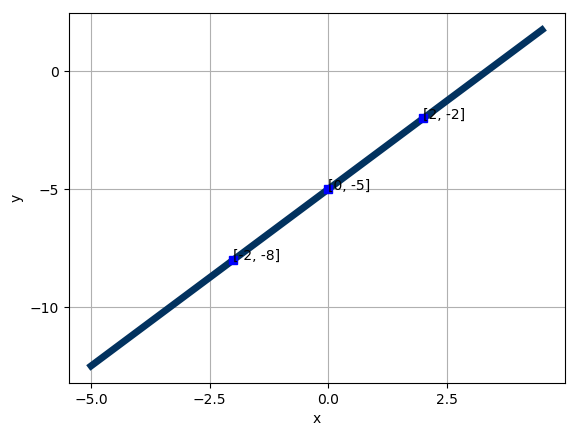
\includegraphics[width=.5\textwidth]{../Figures/question7B.png}
	 \end{center}
\hspace*{11mm} $A = $ \framebox(30,20){} \hspace*{20mm} $B = $ \framebox(30,20){} \hspace*{15mm} $C = $ \framebox(30,20){}
	\begin{enumerate}[label=\Alph*.]
		\item $\sage{choices[0]}$
		\item $\sage{choices[1]}$
		\item $\sage{choices[2]}$
		\item $\sage{choices[3]}$
		\item $\sage{choices[4]}$
	\end{enumerate}		

}

\newpage

\begin{sagesilent}
problemNumber = 8
load("../Code/linear/linearParOrPer.sage")
\end{sagesilent}

% TYPE 2 - Construct a line from a parallel/perpendicular line and a point.
\litem{	\sage{displayStem} 
	
	\begin{center} 
		\sage{lineType} to $\sage{standardFormParOrPer} = \sage{cCoeffInt}$ and passing through the point $(\sage{point[0]}, \sage{point[1]}).$
	\end{center} 
\hspace*{8mm} $m = $ \framebox(30,20){} \hspace*{8mm} $b = $ \framebox(30,20){}
	\begin{enumerate}[label=\Alph*.]
		\item $\sage{choices[0]}$
		\item $\sage{choices[1]}$
		\item $\sage{choices[2]}$
		\item $\sage{choices[3]}$
		\item $\sage{choices[4]}$
	\end{enumerate}
%	\vspace*{-5mm}
}

%OBJECTIVE 2 - Solve linear equations.
\begin{sagesilent}
problemNumber = 9
load("../Code/linear/solveIntegerLinear.sage")
\end{sagesilent}
% TYPE 1 - Solving Basic linear equations (no fractions)

\litem{ \sage{displayStem} 

%$\sage{displayProblem}$
	$$ \sage{blocks[0]}(\sage{blocks[1]+blocks[2]*x}) = \sage{blocks[3]}(\sage{blocks[4]*x-blocks[5]}) $$
\hspace*{10mm} $x = $ \framebox(30,20){} 
	\begin{enumerate}[label=\Alph*.]
		\item $\sage{choices[0]}$
		\item $\sage{choices[1]}$
		\item $\sage{choices[2]}$
		\item $\sage{choices[3]}$
		\item $\sage{choices[4]}$
	\end{enumerate}	
}

% TYPE 2 - Solving Advanced linear equations 
\begin{sagesilent}
problemNumber = 10
load("../Code/linear/solveRationalLinear.sage")
\end{sagesilent}

\litem{ \sage{displayStem}

%$\sage{displayProblem}$

	$$ \frac{\sage{coefficients[0] * x + numerators[0]}}{\sage{denominators[0]}} - \frac{\sage{coefficients[1] * x + numerators[1]}}{\sage{denominators[1]}} = \frac{\sage{coefficients[2] * x + numerators[2]}}{\sage{denominators[2]}} $$
	\hspace*{10mm} $x = $ \framebox(30,20){} 
	\begin{enumerate}[label=\Alph*.]
		\item $\sage{choices[0]}$
		\item $\sage{choices[1]}$
		\item $\sage{choices[2]}$
		\item $\sage{choices[3]}$
		\item $\sage{choices[4]}$
	\end{enumerate}	
	\vspace*{-5mm}
}

\end{enumerate}

\end{document}